\chapter{Conclusions}\label{cap:Conclusions}
In this chapter, we want to give the reader some kind of perception about the feedback from experiments with our program, and suggest future possible improvements.

\section{Results}
To have a perception of how much every step of the algorithm influences the outcome, we will concentrate on a particular trajectory file, and will add ``pieces'' of the algorithm time by time.

First thing first, have a look at figure \ref{fig:corridor_truth}.
In this image, we show the data association that the algorithm performs when running on the ``real'' version of the data (no noise affects odometry and bearing measurements).
In the simulation, there actually was one more landmark, but the important fact is that the algorithm didn't compute wrong associations.

\begin{figure}[htbp]
  \centering
    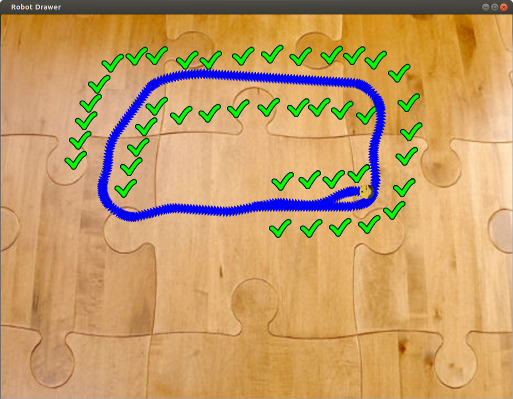
\includegraphics[width=0.3\textwidth]{images/corridor/corridor_truth.png}
  \caption{Trajectory 1 - algorithm run on the ``true'' data values.}
  \label{fig:corridor_truth}
\end{figure}

Ideally, the algorithm should manage to obtain the same map analyzing the noised data.
It's obviously not possible, but we will show how it gets close to the solution. 

Figure \ref{fig:corridor_nooptim} shows the map output of the program when running on the noised data, with optimization inhibition. This means that the odometry guess is taken ``as it is'', and landmark positions are the results of measurements tracking given the robot positions. The solution is evidently ``far'' from the real one.
\begin{figure}[htbp]
  \centering
    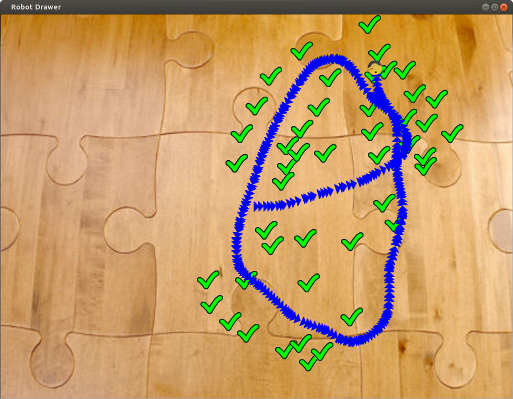
\includegraphics[width=0.3\textwidth]{images/corridor/corridor_nooptim.png}
  \caption{Trajectory 1 - algorithm run on noised data. No optimization is performed.}
  \label{fig:corridor_nooptim}
\end{figure}

Letting the algorithm perform optimizations (both while running and at the end) leads to the result in figure \ref{fig:corridor_optim}. This is in a certain way ``better'' then the previous one, since the landmarks disposition is tidier, but we still didn't improve the trajectory extimation appreciably.
\begin{figure}[htbp]
  \centering
    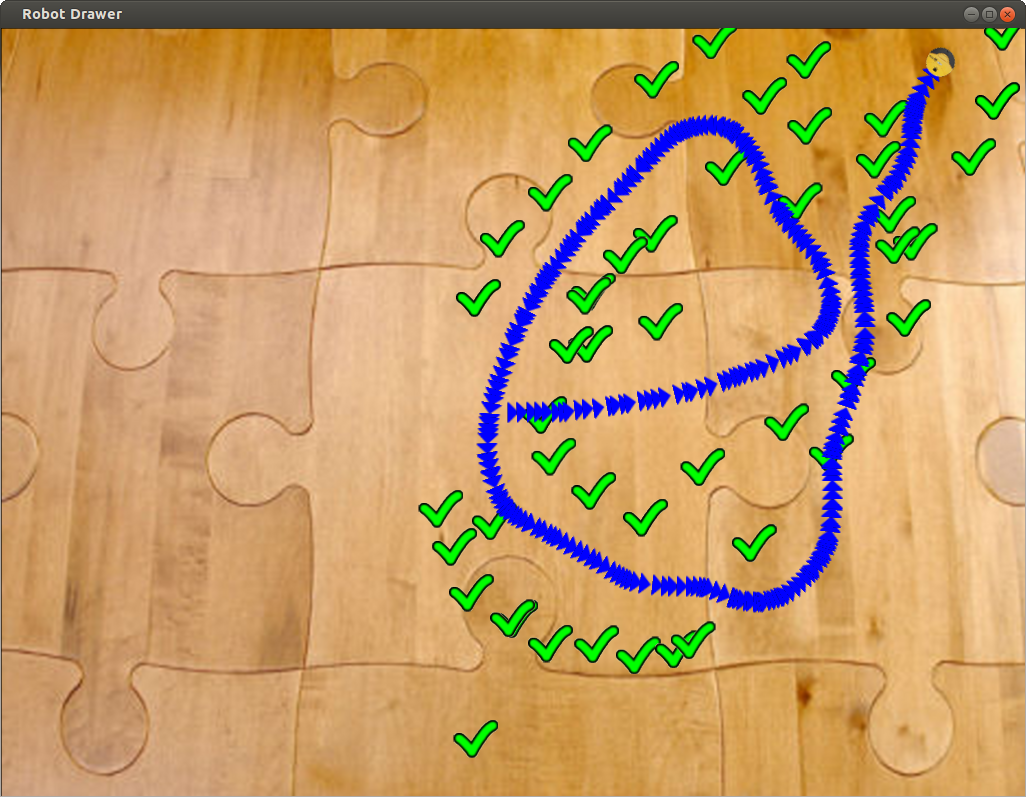
\includegraphics[width=0.3\textwidth]{images/corridor/corridor_optim.png}
  \caption{Trajectory 1 - 30 optimization steps performed every 50 trajectory steps.}
  \label{fig:corridor_optim}
\end{figure}

The final step is to perform ``expectation maximization'', that is to rerun the algorithm taking the newly computed robot positions as initial guess. Each algorithm rerunning (usually) brings the found solution closer to the real one. In figure \ref{fig:corridor_em} you can see the result of rerunning the algorithm about 10 times. The trajectory shape has been approximatively rebuilt, and landmarks arrangement is somehow similar to the original one.
\begin{figure}[htbp]
  \centering
    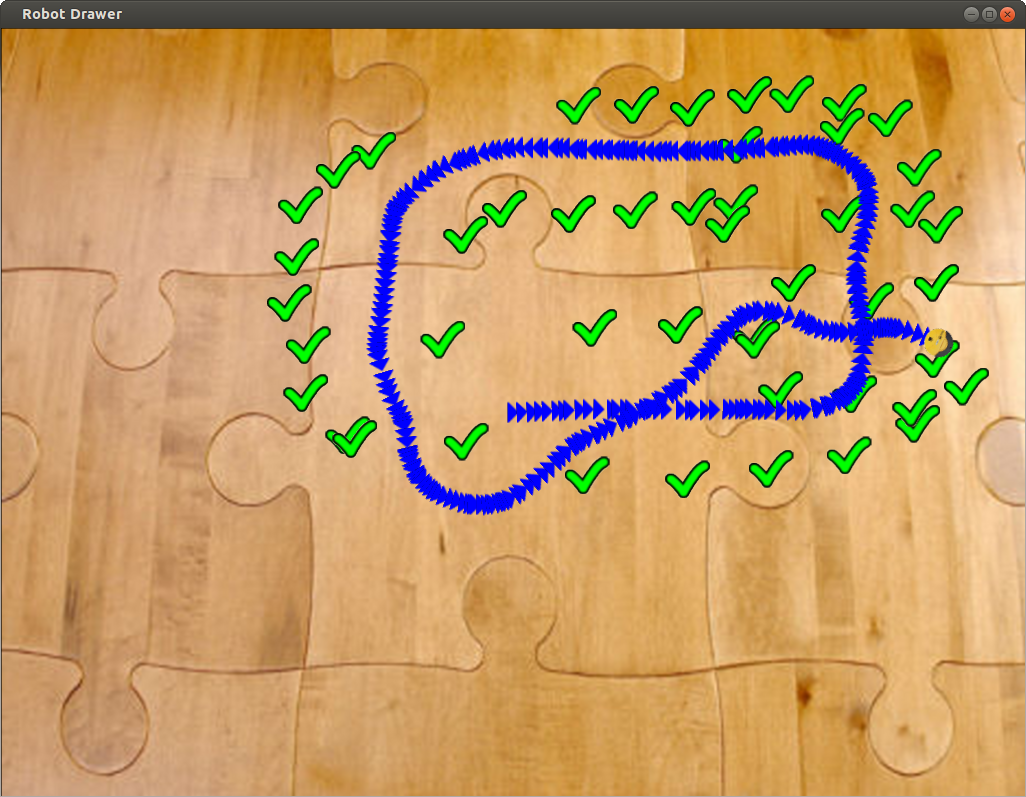
\includegraphics[width=0.3\textwidth]{images/corridor/corridor_rerun10.png}
  \caption{Trajectory 1 - Map produced after some rerunning of the algorithm.}
  \label{fig:corridor_em}
\end{figure}

Figure \ref{fig:corridor2} shows the results on another experiment. In this case, within five rerunning, the algorithm produces a map where the overall rotation has been lost, but the trajectory shape has been reconstructed (note how the robot re-enters inside the corridor after a tour).
\begin{figure}[htbp]
  \centering
    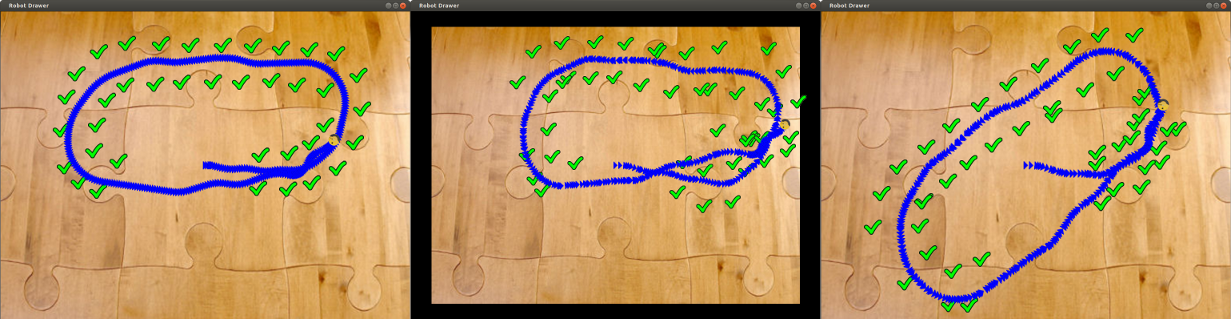
\includegraphics[width=0.9\textwidth]{images/corridor/corridor2.png}
  \caption{Trajectory 2 - [left, true data] [center, only data association] [right, after 5 rerunning].}
  \label{fig:corridor2}
\end{figure}

\section{Future developments}
There are several ideas we got about improvements and future developments about the project:
\begin{itemize}
  \item Optimization phases currently consist of a fixed number of optimization. It would be good to consider optimizing up to when the ``average transformation'' is below a certain threshold.
  \item It would be the case of trying different solvers.
  \item Dinamically variate the number of steps needed to trigger an optimization phase. Contextually, find a convenient way for tuning this number.
  \item Variate the information matrix associated to each edge, according to some criteria to be defined, for instance on the basis of the ``reliability'' of a landmark.
  \item Add the ``closure'' check to the workflow of the algorithm.
  \item Consider using landmarks overlapping to generate new constraints.
  \item Try the program on data from the real world and examine its performances.
\end{itemize}

It would be very nice if, including some of these ideas in the project, we would obtain a system for mapping via as few informations as a bearing. Sounds quite a challenge, but even the results we had look pretty encouraging as a starting point.
